\documentclass[11pt]{article}
\usepackage[margin=1in, paperwidth=8.5in, paperheight=11in]{geometry}
\usepackage{epstopdf}
\usepackage[parfill]{parskip}
\usepackage[pdftex]{graphicx}
\usepackage{changepage}
\usepackage{titling}
\usepackage{amsmath}
\usepackage{amssymb}
\usepackage{bm}
\usepackage{extramarks}
\usepackage{multirow}
\usepackage{amsfonts}
\usepackage{amsthm}
\usepackage{array}
\usepackage{framed}
\usepackage{mathtools}
\usepackage{xy}
\usepackage{hyperref}
\usepackage{float}
\usepackage{subfig}
\usepackage[algoruled]{algorithm2e}
\textwidth 7.0in
\usepackage{fancyhdr}
\usepackage{lastpage}
\pagestyle{fancy}
\fancyhf{}
\linespread{1.1}
\newcommand{\inlinecode}{\texttt}
\newcommand{\divider}{\line(1,0){250}}
\rfoot{Page \thepage \  of \pageref{LastPage} }

\renewcommand\headrulewidth{0.4pt}
\renewcommand\footrulewidth{0.4pt}

\newcommand{\specialcell}[2][c]{%
  \begin{tabular}[#1]{@{}c@{}}#2\end{tabular}}

\setlength\parindent{0pt}

\hypersetup{
    colorlinks=true,
    linkcolor=black,
    filecolor=magenta,      
    urlcolor=blue,
    citecolor=blue
}

%Custom definitions
\newcommand{\problempart}[1]{\textbf{#1.}}
\newcommand{\pof}[1]{\text{P(#1)}}
\newcommand{\subtitle}[1]{%
      \posttitle{%
              \par\end{center}
                  \begin{center}\large#1\end{center}
                          \vskip0.5em}%
                      }

%%Set symbols
\newcommand{\given}{\ensuremath{|} }
\newcommand{\AND}{\ensuremath{\cap} }
\newcommand{\OR}{\ensuremath{\cup} }

\newcommand{\N}{\mathbb{N}}
\newcommand{\R}{\mathbb{R}}
\newcommand{\Z}{\mathbb{Z}}
\newcommand{\Q}{\mathbb{Q}}

\newcommand{\powerset}[1]{\ensuremath{ \mathcal P \left({#1}\right)}}
\newcommand{\set}[1]{\ensuremath{\left\{ #1 \right\}}}
\newcommand{\stcomp}[1]{\overline{#1}} 

\newcommand{\dlim}[2][\infty]{\displaystyle \lim_{#2 \rightarrow #1}}
\newcommand{\indefint}{\displaystyle \int}
\newcommand{\be}{\begin{enumerate}}
\newcommand{\ee}{\end{enumerate}}
\newcommand{\dsum}[2]{\displaystyle \sum_{#1}^{#2} }
\newcommand{\defint}[4]{\int^#2_#1 #3\,d#4}

\newcommand{\bx}{\ensuremath{\mathbf{x}}}
\newcommand{\bz}{\ensuremath{\mathbf{z}}}
\newcommand{\bphi}{\ensuremath{\bm{\phi}}}
\newcommand{\kl}[1]{\textsc{kl}\left(#1\right)}
\newcommand{\g}{\,\vert\,}

\newcommand{\EE}[1]{\mathbb{E}\left[#1\right]}
\newcommand{\EEE}[2]{\mathbb{E}_{#1}\left[#2\right]}
\newcommand{\ELBO}{\textsc{elbo}}

\newcommand{\defeq}{\stackrel{.}{=}}

% Various Helper Commands
%

\newcommand{\adjustimg}{% Horizontal adjustment of image
  \checkoddpage%
  \ifoddpage\hspace*{\dimexpr\evensidemargin-\oddsidemargin}\else\hspace*{-\dimexpr\evensidemargin-\oddsidemargin}\fi%
}
\newcommand{\centerimg}[2][width=\textwidth]{% Center an image
  \makebox[\textwidth]{\adjustimg\includegraphics[#1]{#2}}%
}


% Useful for algorithms
\newcommand{\alg}[1]{\textsc{\bfseries \footnotesize #1}}

% For derivatives
\newcommand{\deriv}[1]{\frac{\mathrm{d}}{\mathrm{d}x} (#1)}

% For partial derivatives
\newcommand{\pderiv}[2]{\frac{\partial}{\partial #1} (#2)}

% Integral dx
\newcommand{\dx}{\mathrm{d}x}

% Alias for the Solution section header
\newcommand{\solution}{\textbf{\large Solution}}

% Probability commands: Expectation, Variance, Covariance, Bias
\newcommand{\E}{\mathrm{E}}
\newcommand{\Var}{\mathrm{Var}}
\newcommand{\Cov}{\mathrm{Cov}}
\newcommand{\Bias}{\mathrm{Bias}}
\newcommand\mc[1]{\multicolumn{1}{c}{#1}}
\newcommand{\matr}[1]{\mathbf{#1}}

\makeatletter
\def\thm@space@setup{%
  \thm@preskip=0.4cm
  \thm@postskip=\thm@preskip % or whatever, if you don't want them to be equal
}
\makeatother


\newtheorem{theorem}{Theorem}
\newtheorem{lemma}{Lemma}
\newtheorem{proposition}{Proposition}
\newtheorem{observation}{Observation}
\newtheorem{proposal}{Proposal}
\newtheorem{claim}{Claim}
\newtheorem*{problem*}{Problem}

\SetKwComment{Comment}{$\triangleright$\ }{}

% Move qed box to the left
\renewcommand{\qed}{\unskip\nobreak\quad\qedsymbol}

\newenvironment{conditions}
  {\par\vspace{\abovedisplayskip}\noindent\begin{tabular}{>{$}l<{$} @{${}={}$} l}}
  {\end{tabular}\par\vspace{\belowdisplayskip}}

% Title page

  \title{\vspace{2in}Clustering SNVs for Tumor Heterogeneity}
  \subtitle{Brown University, Math-CS Sc.B Thesis}
  \date{ \vspace{1.0in} \today}
\author{David Liu \vspace{1.5in}\\ Supervisor: Professor Ben Raphael \\[20pt] Reader: Professor Erik Sudderth}

% Header
\begin{document}
\maketitle
\newpage
\tableofcontents
\section{Introduction}
Cancer results from an evolutionary process where somatic mutations occur and accumulate in a population of cells. There are many types of mutations that can cause cancer. A mutation that causes genetic variation at a single genomic site is called a \emph{single nucleotide variant (SNV)}. The different lineages which comprise a tumor are known as clones, and the phenomenon of clonal admixture is known as intratumor heterogeneity \cite{Nowell1976}. The relation of clones with each other is best visualized with a phylogenetic tree, since mutations accumulate within and across subpopulations.

\begin{figure}[h]
\par
\raisebox{-.5\height}{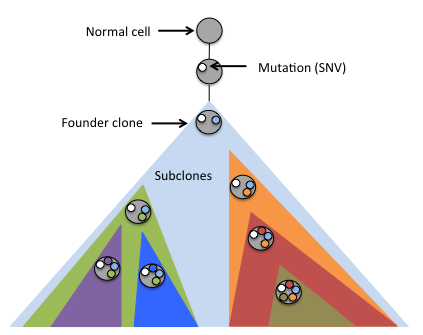
\includegraphics[width=3.5in]{heterogeneity.png}}%
%\hfill
\hspace{0.5in}
\raisebox{-.5\height}{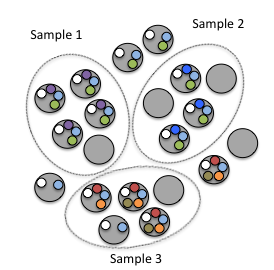
\includegraphics[width=3in]{multiplesamples.png}}%
\par
\caption{\emph{Left: Example of a clonal tree caused by tumor heterogeneity. Right: Spatial samples from a tumor. Figure from} \cite{Ancestree}.}
\label{fig:Heterogeneity}
\end{figure}

The sequencing and analysis of tumors has revealed extensive intratumor heterogeneity in cancers. This is a clinically relevant problem, as the genetic profile of a tumor can lead to treatment failure and drug resistance; increased tumor heterogeneity has been linked with more aggressive cancers \cite{Gerlinger2012}. The ability to genetically profile a tumor would improve physicians' ability to tailor treatments according to the subpopulations and mutations present \cite{Raphael2014}. 

One of the most studied problems in tumor heterogeneity is tree inference, in which we estimate the evolutionary history and mixing proportions of clones \cite{Ancestree}. A clone is typically defined as a group of cells that arose from the same set of mutations, so that the cells with this  In doing so, we must know which mutations belong to each clone---to have a tree, we must know what the constituent nodes are. This problem is made more tractable by incorporating multiple samples from the tumor (eg. biopsies separated physically or temporally), which provides more information for inference, since the clonal membership of SNVs is invariant across samples. We view the problem of assigning mutations to clones as a general machine clustering problem.

\section{General Model}
\subsection{Variant Allele Frequency}
The data typically used for tree inference is called the \emph{variant allele frequency (VAF)}, which is a measure of how much a mutation occurs in a population. The VAF is determined by sequencing a sample from a tumor, so that the reads represent the sample's mixture of clones \cite{Ding2012}. By comparing to a control sample, if a read contains the mutated allele at a SNV, it is called a variant read; otherwise it is called a reference read. The VAF is defined for each SNV in each sample, as, in each sample, the number of variant reads at an SNV divided by the number of total reads at that SNV. Across multiple samples, each mutation that belongs to a clone should be observed to have about the same variant allele frequency, because the clone frequency is the same; thus a clustering should be true for each clone across all samples.

\subsection{Clonal Membership and Generation of Reads}
We can express the mathematical dependencies in our model in terms of the processes that generate them: SNVs (labels) are assigned to clones (clusters), and variant reads are generated according to clone-specific parameters. From here on, we will use SNVs to refer to labels, and we will use clusters to refer to clones.

First, each SNV $n \in \{1, ..., N\}$ belongs to a cluster $k\in\{1,\ldots,K\}$, $K \leq N$. Note that we do not know the true number of clusters in advance, since the cancer mutates unpredictibally. These cluster memberships are described by the latent variables $\bz_n$, a 1-of-$K$ indicator vector that denotes the cluster assignment of SNV $n$ to cluster $k$. 

Now suppose that for each sample $m\in\{1, \ldots M\}$, we have total reads $d_{mn}$ drawn from a Poisson with expected value equal to the coverage \cite{Lander1988}. Let SNV $n$ belong to cluster $k$. Then variant reads $v_{mn}$ are generated according to distribution $V(v_{mn}; d_{mn}, \bphi_{mk})$, where $V$ is any probability distribution that depends on $v_{mn}$ and has parameters $d_{mn}, \bphi_{mk}$. By vectorizing, we can make clear that the clustering for a SNV $n$ is fixed across samples $m$.
\begin{align}
\bm{d_{n}} &= 	\begin{bmatrix} d_{1n} \\ d_{2n} \\ \vdots \\ d_{Mn} \end{bmatrix}, \quad\bm{v_{n}} = 	\begin{bmatrix} v_{1n} \\ v_{2n} \\ \vdots \\ v_{Mn} \end{bmatrix}	\\[20pt]
	\bf{v}_{n} &\defeq 
				\begin{bmatrix}
				 	v_{1n} \\ v_{2n} \\ \vdots \\ v_{Mn}
				\end{bmatrix}
				\sim
				\begin{bmatrix}
					V(v_{1n}; d_{1n}, \bphi_{1k}) \\ V(v_{2n}; d_{2n}, \bphi_{2k}) \\ \vdots \\ V(v_{Mn}; d_{Mn}, \bphi_{Mk})
				\end{bmatrix}
				\defeq \bm{V(\bphi_k)}
\end{align}

Let $\bx_{n}$ be general notation for $\{\bm{d}_{n}, \bm{v}_{n}\}$, where the use of the reference or variant reads will be clear from context. Generalizing notation further, let $\bx = \{\bx_1, \ldots, \bx_n\}$, $\bphi = \{\bphi_1, \ldots, \bphi_n\}$, and $\bz = \{\bz_1, \ldots, \bz_n\}$. Then we wish to discover the underlying $\bz, \bphi$ for the model given some observations $\bx$.

\begin{problem*}[SNV clustering problem]
Suppose that for SNVs $n \in \{1, ..., N\}$ in samples $m\in\{1, \ldots M\}$. Further suppose that there exists clones (clusters) $k\in\{1,\ldots,K\}$ and a true clustering $\bz$. Given total reads $\bm{d}_1, \ldots, \bm{d}_n$ and variant reads $\bm{v}_1, \ldots, \bm{v}_n$, how can we recover the $\bm{z}$ and $\bphi$?
\end{problem*}

\section{Existing methods}

There are existing clustering methods in bioinformatics such as SciClone, Clomial, and PyClone \cite{SciClone, Clomial, PyClone}. These methods follow the model described above; two popular choices for $V$ are the binomial and beta distributions. The binomial distribution is a natural choice due to the binary nature of read data. It is also attractive because the number of reads which belong to a cluster naturally weighs the cluster's mixing proportion, which is not necessarily true for the beta model. The beta distribution is also a natural choice for $V$ because variant allele frequencies are in the range $(0,1)$. That is, $V$ is beta with data $f_{mn} = \frac{v_{mn}}{d_{mn}}$. 

However, these methods differ in model selection and inference. For example, SciClone uses a fixed number of clusters through a Dirichlet prior and an ad-hoc heuristic for $K$, with inference through variational inference. Clomial uses a Dirichlet prior and the BIC for model selection, and EM for inference. PyClone uses a Dirichlet Process prior, and MCMC for inference. Thus PyClone has the same model, but uses a slower inference technique.

State of the art clustering methods use the Dirichlet process to select the number of clusters, which as a nonparametric model, can provide more rigorous model selection. There is also a need for inference on large datasets, for which variational inference is useful. MCMC, while accurate in the long run, may have poor convergence properties, while variational inference is a faster technique that potentially trades off some accuracy for speed and scalability \cite{Jordan1999}. In this thesis, I attempt to augment existing approaches by proposing and implementing a method to cluster mutations using variational inference for a binomial mixture model with Dirichlet process prior, which is suited for the multi-sample clone mixing problem.

\begin{table}[ht]
  \large
  \centering
  {\renewcommand{\arraystretch}{1.5}
  \begin{tabular}{c|c|*{2}{c|}}
    \multicolumn{2}{c}{} & \multicolumn{2}{c}{Model Selection} \tabularnewline
    \cline{2-4}
    \multirow{3}*{\rotatebox{90}{Inference Method}} 
&    \bfseries  & \bfseries \specialcell{Dirichlet Prior + Heuristic \\ (Fixed $K$)} & \bfseries \specialcell{Dirichlet Process Prior\\ (countably infinite $K$)}  \tabularnewline[1 ex] 
\cline{2-4}
&    \bfseries MCMC & (Many older methods)  & PyClone  \tabularnewline [1ex] 
    \cline{2-4}
&    \bfseries VI & SciClone  & \emph{This thesis} \tabularnewline [1ex] 
    \cline{2-4}
  \end{tabular}
  }
  \caption{A comparison of methods used to solve the clonal mixture problem.}
   \label{table:methods}
\end{table} 

\newpage

\section{Binomial Mixture Model with DP prior}
Figure~\ref{fig:GM} on the next page shows a graphical model representation of the model.

Suppose that each clone in each sample emits variant reads according to a binomial distribution. Thus, for cluster $k$, some SNV $n$ which belongs to this cluster, and reads $d_{mn}$, we have variant reads distributed according to $\mathrm{Bin}(v_{mn}; d_{mn}, \bphi_{mk})$. Call $\phi_{mk}$ the cluster frequency for sample $m$ in cluster $k$. By the independence of reads across samples, the joint probability of reads for an SNV is the product across all samples. Using our vectorized notation,
\begin{equation} \label{eq:xlikelihood}
\Pr(\mathbf{x_n} | \bphi_k) = \prod\limits_{m=1}^M \mathrm{Bin}(v_{mn}; d_{mn}, \bphi_k)
\end{equation}

Let the cluster memberships $\bz_n$ and weights $\pi_k$ be generated by a Dirichlet process prior. The reader is referred to \cite{Antoniak1974} for more mathematical detail on the DP. By truncating the DP at $K = N$, $K \in \{1, \ldots, N\}$ with probability 1.

The likelihood of $\bx_n$ depends on the latent variables in a straightforward way from (\ref{eq:xlikelihood}):
\begin{align} \label{eq:jointlikelihood}
\Pr(\mathbf{x_n} | \bz, \bphi_k) &= \prod\limits_{k=1}^K \Pr(\mathbf{x_n} | \mathbf{\phi_k})^{\bz_{nk}} \nonumber \\
										&= \prod\limits_{k=1}^K \prod\limits_{m=1}^M \mathrm{Bin}(v_{mn}; d_{mn}, \bphi_{mk})^{\bz_{nk}}
\end{align}
Then the joint likelihood of the observed data and cluster memberships, follows from (\ref{eq:jointlikelihood}): 
\begin{equation}
\Pr(\mathbf{x_n}, \bz | \bm{\pi}, \bphi) = \prod\limits_{k=1}^K \prod\limits_{m=1}^M \left(\pi_k \mathrm{Bin}(v_{mn}; d_{mn}, \phi_{mk})\right)^{\bz_{nk}}
\end{equation}

As described in \cite{Blei2006}, the Dirichlet Process can be described constructively with a stick-breaking process as follows, for some base measure $H$ and concentration parameter $\alpha$:
\begin{align}
\pi_i(\mathbf{v}) &= v_i \prod\limits_{j=1}^{i-1} (1 - v_j) \\
				DP &= \sum_{i=1}^\infty \pi_i(\mathbf{v}) \delta_{\phi_i}
\end{align}
\begin{enumerate}
	\item Draw $v_k | \alpha \sim \mathrm{Beta}(1, \alpha)$, \hspace{0.2cm} $k = \{1, 2, \ldots\}$
	\item Draw $\bphi_k | H \sim H^M$, \hspace{1cm} $k = \{1, 2, \ldots\}$
	\item For the $n$th data point:
	\begin{enumerate}
		\item Draw $z_n | \{\pi_1, \pi_2, \ldots\} \sim \mathrm{Cat}(\pi(\mathbf{v}))$.
		\item Draw $\bx_n | z_n \sim p(\bx_n | \bphi_k)$.
	\end{enumerate}
\end{enumerate}
The full cluster assignment posterior 
\begin{equation}
p(\bz | \bx, \alpha, H) = \int p(\bx | \mathbf{\phi}) p(\phi | \bx, \alpha, H) \, d\phi
\end{equation}
involves a Dirichlet Process and is thus analytically intractable. We must use some sort of computational technique, such as variational inference, to perform inference on this posterior.

\begin{figure}[h]
\centerimg[scale=1.0]{multi_pgm.png}
\caption{Graphical model for the VAFs.}
\label{fig:GM}
\end{figure}

\begin{quote}
$n = 1, \ldots , N$:  SNVs \\
$m = 1, \ldots , M$: samples \\
$k = 1, \ldots ,  K$: clusters
\end{quote}

\begin{quote}
$\alpha$ = Hyperparameter for the stick-breaking process \\[2pt]
$H \sim U(0,1) \sim \mathrm{Beta}(1, 1)$ = Base distribution for cluster frequencies ($\phi_{mk}$)	 \\[2pt]
$\pi_k$ =  Cluster weights, generated from the stick-breaking process \\[2pt]
$z_{n} \in \{1, \ldots, K, \ldots \}  \sim \mathrm{Cat}_\infty(\pi_1, \ldots, \pi_K, \ldots)$ =  Cluster membership for SNV $n$\\[2pt]
$\phi_{mk}$ = Cluster frequency \\ [2pt]
$v_{mn} \sim \mathrm{Binom}(v_{mn}; d_{mn}, \phi_{mk})$ = {\smaller Observed variant reads for sample $m$, SNV $n$, belonging to cluster $k$.} \\ [2pt]
$d_{mn} \sim \mathrm{Pois}(\text{Coverage})$ = Observed total reads for sample $m$, SNV $n$
\end{quote}
\vspace{0.05cm}


\section{Overview of Variational Inference}

\emph{Variational inference} (VI) is an alternative to MCMC-based inference methods. At a high level, variational inference factors a posterior using the mean-field approximation, which approximates the posterior in a higher-dimensional space using simpler independent functions. Then a simple coordinate ascent can be performed in order to infer the model parameters. The following is a general treatment of VI, where latent variables refer to cluster memberships.

\subsection{The \textsc{ELBO}}

The following is from \cite{Blei2006}. Let $\mathbf{z}$ denote the latent variables, and $\mathbf{x}$ denote the data. We seek to approximate the posterior $p(\mathbf{z}|\mathbf{x})$ from a family of distributions $\mathcal{D}$ by solving the following optimization problem: 
\begin{equation} \label{eq:optimalq}
q^*(z) = \arg\!\min_{q(\mathbf{z}) \in \mathcal{D}} \kl{(q(\mathbf{z}) || p(\mathbf{z}|\mathbf{x}))}.
\end{equation}

where \textsc{kl} is the KL-divergence, which measures the ``distance'' between two distributions. 

However, (\ref{eq:optimalq}) requires us to compute the log evidence (which is intractable over the space of all $\mathbf{z}$) since 
\begin{align}
  \kl{q(\bz) \| p(\bz \g \bx)} =
  \E\left[\log q(\bz)\right] -
  \E\left[\log p(\bz, \bx)\right] +
  \log p(\bx). 
\end{align}

Instead, we optimize an objective function which is not dependent on $\log p(\bx)$. We call this the evidence lower bound (\textsc{ELBO}), which is equal to the negative \textsc{KL}-divergence plus the $\log$ evidence.
\begin{align} \label{eq:ELBO}
  \ELBO(q) =
  \E{[\log p(\bz, \bx)]} -
  \E{[\log q(\bz)]}.
\end{align}
and thus we see that $\log p(\bx)$ is a constant with respect to $q$. The $\textsc{ELBO}$ gets its name from the fact that it is a lower bound for the $\log$ evidence. 

\subsection{The mean-field variational family}
The standard technique is to select a simple family of distributions for $\mathcal{D}$, the mean-field variational family \cite{Blei2006}. In this family, the latent variables $\bz$ are mutually independent so that the joint distribution factorizes:
\begin{align} \label{eq:meanfield}
  q(\bz) = \prod_{j=1}^{m} q_j(z_j).
\end{align}
where $q_j$ is a bounded variation dependent only on $z_j$. The structure of the model will dictate the optimal form of $q_j$. 

\subsection{Coordinate ascent}
The optimization is solved using a coordinate ascent algorithm, where via the mean-field assumption, the independence of the latent variables gives us something similar to orthogonality. Let $\bz_{-j}$ denote the set of latent variables $\bz_l$ such that $l \neq j$. Consider the complete conditional probability of $z_j$, which is a function of the other latent variables and the data, $p(z_j \g \bz_{-j}, \bx)$. Since the expectation in the \textsc{ELBO} is with respect to $q(\bz)$, which we have assumed factorizes, then we can dissect out the dependence \cite{Bishop2006} with respect to $\bz_j$ by using (\ref{eq:ELBO}) and (\ref{eq:meanfield}):
\begin{align}
\ELBO(q) &= \int \prod q_i(\bz_i) \left(\log p(\bz, \bx) - \sum_i \log q_i(\bz_i) \right) \,d\bz \nonumber \\
			&\propto \int q_j(z_j) \E_{-j}\left[\log p(\bx, \bz) \right] \, d\bz_j - \int q_j(z_j) \log q_j(\bz_j) \, d\bz_j
\end{align}
Now suppose that we fix $z_{-j}$ and maximize the \textsc{ELBO}. Then the \textsc{ELBO} is maximized when $\log q_j(\bz_j) \propto \E_{-j}\left[\log p(\bx, \bz) \right]$, by the positivity of the $\textsc{KL}$-divergence. Thus the optimal $q^*(\bz_j)$ occurs when
\begin{align} \label{eq:coordascent}
q^*_j(\bz_j) \propto \exp\left(\E_{-j}\left[\log p(\bx, \bz) \right]\right)
\end{align}

(\ref{eq:coordascent}) underlies the coordinate-ascent variational inference algorithm. By iterating through each variational factor, fixing the others, and performing coordinate ascent (similar to Gibbs sampling), then we eventually reach a local optimum of the \textsc{ELBO}.

\subsection{Exponential family distributions yield a general formula}

If the posterior is in the exponential family, then the computation of coordinate ascent and ELBO can be generalized. Recall that a distribution is in exponential form if it can parameterized by 
\begin{equation}
f_X(x\mid\theta) = h(x) \exp \left (\theta^T \cdot T(x) -A(\theta)\right )
\end{equation}
where $T(x)$ is the sufficient statistic vector, $\theta$ is the natural parameter vector, and $A(\theta)$ is the cumulant. The details are in \cite{Hughes2015}, but the intuition is that because the optimal variational updates (\ref{eq:coordascent}) are proportional to $\exp(\E[\log(.)])$ then writing the distribution in exponential form reveals dependencies that hold for all exponential family members.


\section{Variational Inference on DP Binomial Model}
Now we apply the variational inference framework to the model we developed.

\subsection{The model and its ELBO}

We write the ELBO as a function of the data and latent variables:
\begin{equation}
	\begin{split}
		\ELBO\left(q(\bx, \bz | \gamma, \alpha_0, \beta_0)\right) = &E_q[\log p(\mathbf{v} | \gamma)] + E_q[ \log p(\bm{\phi} | \alpha_0, \beta_0)] + \\ &\sum\limits_{n=1}^N \left( E_q[\log p(z_n | \mathbf{v})] + E_q[\log p(x_n | z_n)]\right) \\  &- E_q[\log q(\bz, \mathbf{v}, \bm{\phi})]
	\end{split}
\end{equation}
where $\lambda$ represents the hyperparameter governing the stick-breaking process, and $\alpha_0, \beta_0$ are the hyperparameters governing the base beta distribution. By the mean-field assumption, the joint distribution for the last term in the $\ELBO$ factors as follows:
\begin{align}
    q(\bz, \mathbf{v}, \bm{\phi}) &=
\underbrace{\prod\limits_{k=1}^K q(\bm{\phi}_k)}_{\substack{\text{Observation: likelihoods}  \\  \text{Product of betas} \\ 2MK \text{ variational parameters} \\  \{\alpha_{mk}, \beta_{mk} \}_{m=1, k=1}^{M, K} }} \times
 \underbrace{\prod\limits_{k=1}^K q(\mathbf{v}_k)}_{\substack{\text{Allocation: cluster proportions} \\ \text{Product of betas} \\ 2K \text{ variational parameters}  \\ \{\eta_{k0}, \eta_{k1}\}_{k=1}^K   }} \times
 \underbrace{\prod\limits_{n=1}^{N} q(z_n)}_{\substack{ \text{Allocation: cluster responsibilities} \\ \text{Product of categoricals} \\ 2NK \text{ variational parameters}  \\ \{\hat{r}_{nk}\}_{n=1, k=1}^{N, K}   }} \nonumber
\end{align}

Note that the cluster proportions and data assignments are dictated by the Dirichlet Process|we call this the allocation model. On the other hand, the observation parameters vary depending on the structure of the generative model|we call this the observation model (Hughes 2015). Here we derive the form of the  $q(\bm{\phi}_k)$ is a function of $\bm{\phi_k}$, as the observation model is specific to our multi-sample binomial model.

We note that for an individual allelic site in a sample, the data likelihood is binomial. With a beta prior, we know that the resulting posterior for $q(\bm{\phi}_{mk})$ is conjugate to the binomial, and thus $q(\bm{\phi}_{mk}) \sim \mathrm{Beta}(\bm{\phi}_k | \alpha_{mk}, \beta_{mk})$ where $\alpha_{mk}, \beta_{mk}$ are variational parameters. Because reads across samples at a site are assumed to be independent, then we have 
\begin{align*}
q(\bm{\phi}_k)  &= \prod\limits_{m=1}^M q(\bm{\phi}_{mk}) \\
				&= \prod\limits_{m=1}^M \mathrm{Beta}(\bm{\phi}_k | \alpha_{mk}, \beta_{mk})
\end{align*}

\subsection{Coordinate ascent algorithm}

The derivations of the coordinate ascent algorithm are in Appendices A and B. The derivations for the ELBO are in Appendix C. We have the following procedure for coordinate ascent on our model.

\subsubsection{Initialization}
The initial responsibilities of the cluster were chosen by setting $\hat{r}_{nk} = 1$ if $n$ was set to be in cluster $k$ by the k-means++ algorithm with $N$ initial clusters \cite{Hughes2015}, with the other $\hat{r}_{n.}$ set to be $\frac{1}{k}$. These responsibilities were then normalized. For the other parameters, we assume that they are set to their prior or uniform values. Thus the truncation level of $K$ was set to be $N$, with all $K > N$ having zero probability.

Since we assumed a uniform prior, $\alpha_0 = \beta_0 = 1$. The other parameters were chosen empirically. We let $\gamma_1 = \eta_1 = 1.0$ and $\gamma_0 = \eta_0 = 1.5$.

\subsubsection{Convergence}
We declare the coordinate ascent procedure to be complete when the difference in ELBO between two iterations is less than some convergence threshold. Empirically, we chose the threshold to be equal to 0.01. 

The following pseudocode follows the format of \cite{Hughes2015}.
\begin{algorithm}[h]
\SetCommentSty{itshape}
\KwIn{Data $\bx_n$, where each $x_i$ is an integer vector with $M$ entries. \\ \hspace{1.25cm} $\gamma_0, \gamma_1, \alpha_0, \beta_0$, hyperparameters}
\vspace{0.1cm}
\KwOut{Converged variational parameters $\{\alpha_{mk}, \beta_{mk} \}_{m=1, k=1}^{M, K}, \{\eta_{k0}, \eta_{k1}\}_{k=1}^K, \{\hat{r}_{nk}\}_{n=1, k=1}^{N, K}$}
	\vspace{0.1cm}
\textbf{Initialize:}     $\alpha_0 = \beta_0 = \alpha_{mk} = \beta_{mk} = 1$, $\forall m, k$ \\
\hspace{1.85cm}    $\gamma_1 = \eta_1 = 1.0, \gamma_0 = \eta_0 =1.5$ \\
\hspace{1.85cm}    $\hat{r}_{nk} \leftarrow \texttt{kmeans++}(\bx)$ \\
	\vspace{0.1cm}
\While{the \textsc{ELBO} has not converged} {
	\vspace{0.05cm}
	\Comment*[h]{Compute data-specific (local) parameters} \\
		\hspace{1cm} $\E_q[\log p(x_n | \alpha_{mk}, \beta_{mk})] \leftarrow \E_q[\log \left( \binom{d_{mn} + v_{mn}}{v_{mn}} (\bm{\phi}_k)^{v_{mn}} (1-\bm{\phi}_k)^{d_{mn}} \right)]$ \\
		\hspace{1cm} $\hat{r}_{nk} \leftarrow \exp(S_k)$ \\
		
	\vspace{0.1cm}	
	\Comment*[h]{Compute sufficient statistics} \\
		 \hspace{1cm} $S_k = \sum_{n=1}^N \hat{r}_{nk} s(x_n) = \sum_{n=1}^N \hat{r}_{nk} \begin{bmatrix}
				\begin{bmatrix}
				 v_{1n} &  d_{1n}
				\end{bmatrix} & \cdots &
				\begin{bmatrix}
				 v_{Mn} &  d_{Mn}
				\end{bmatrix}
			\end{bmatrix}$ \\
		\hspace{1cm} $N_k = \sum_{n=1}^N \hat{r}_{nk}$ \\
		\hspace{1cm} $N_k^> = \sum_{k+1}^K N_k$
	
	\vspace{0.1cm}	
	\Comment*[h]{Compute cluster-specific (global) parameters} \\
		\hspace{1cm} $\eta_{k1} \leftarrow 1 + \sum_n \hat{r}_{nk} = 1 + N_k$ \\
		\hspace{1cm} $\eta_{k0} \leftarrow \gamma + \sum_n \sum_{j=k+1}^K \hat{r}_{nj} = N_k^>$\\
%		\hspace{1cm} $[\bm{\alpha}_{k}, \bm{\beta}_{k}] \leftarrow [(\alpha_0 - 1), (\beta_0 - 1)] + S_k $ \\
		\hspace{1cm} $\alpha_{mk} \leftarrow  (\alpha_0 - 1) + S_{km}$ \\
		\hspace{1cm} $ \beta_{mk} \leftarrow (\beta_0 - 1) + S_{km}$ \\
	\vspace{0.1cm}		
  Compute $\ELBO(q) = \EE{\log p(\bz, \bx)} + \EE{\log q(\bz)}$
}
\Return{Converged variational parameters}
\caption{\textsc{CAVI for the multidimensional Binomial model}}
\label{alg:cavi}

\end{algorithm}

\subsection{MAP estimates}
For each cluster we pool reads by cluster membership:
\begin{align}
v_{mk}^{\text{pooled}} &= \sum_n (v_{mn})^{\bz_n} \\
d_{mk}^{\text{pooled}} &= \sum_n (d_{mn})^{\bz_n} \\
\intertext{and we can make MAP estimates by converting from the variational parameters back to the original parameters of the posterior:}
\bz_n^{\text{MAP}} &= \arg \max_k \hat{r}_{nk}  \\[8pt]
\phi_{mk}^{\text{MAP}} &= \frac{v_{mk}^{\text{pooled}} + \alpha_{mk} - 1}{d_{mk}^{\text{pooled}} + \alpha_{mk} + \beta_{mk} - 2}
\end{align}


\subsection{Implementation}
The VI coordinate ascent algorithm was implemented in Python. The code is available \href{https://github.com/daviddliu/thesis/tree/master/clustering}{on Github}.

\section{Experiments and Results}

The coordinate ascent algorithm was benchmarked against SciClone and PyClone, as these are the state-of-the-art methods for the other types of model selection and inference (see Table \ref{table:methods}). These methods were first run on simulated data with the following parameters:

\begin{table}[ht]
\centering
\begin{tabular}{| l | l |}
\hline
Number of clusters ($K$) & 10            \\ \hline
Number of SNVs ($N$)     & 100           \\ \hline
Number of samples ($M$)  & 4, 5, 6       \\ \hline
Coverage                 & 50, 100, 1000  \\ \hline
\end{tabular}
\caption{Parameters for the simulated datasets.}
\label{table:simulateddata}
\end{table}

To evaluate the accuracy of cluster assignments ($\bz^{\text{MAP}}$), we used the adjusted Rand Index (ARI), which is defined in \cite{Rand1971}. The ARI takes as input two clusterings and returns a number in $[0,1]$, where 0 indicates no matches, and 1 indicates that the two clusterings are the same. Thus, for a putative clustering $\mathcal{C}$ and the true clustering $\mathcal{K}$, we are interested in $\textsc{ARI}(\mathcal{C}, \mathcal{K})$.

To evaluate the accuracy of the cluster parameters ($\bphi^{\text{MAP}}$), we define the cluster frequency error (CFE), which is the expected error between the putative cluster parameters $\bphi^{\text{MAP}}_k$ and the true cluster parameters $\bphi_k$ over the putative clusters. Suppose that a clustering algorithm estimates $C$ putative clusters. Then
\begin{align}
\text{CFE}(\bphi^{\text{MAP}}) \defeq  \frac{1}{C} \sum_{c=1}^C \min_{k \in \{1, \ldots, K\}}  \left\Vert \bphi_c^{\text{MAP}} - \bphi_k \right\Vert.
\end{align}

\subsection{Results on simulated data}

\subsection{Results on real data}

\section{Discussion}
+ Compare accuracy between the three methods.

\begin{figure}[h]
\centerline{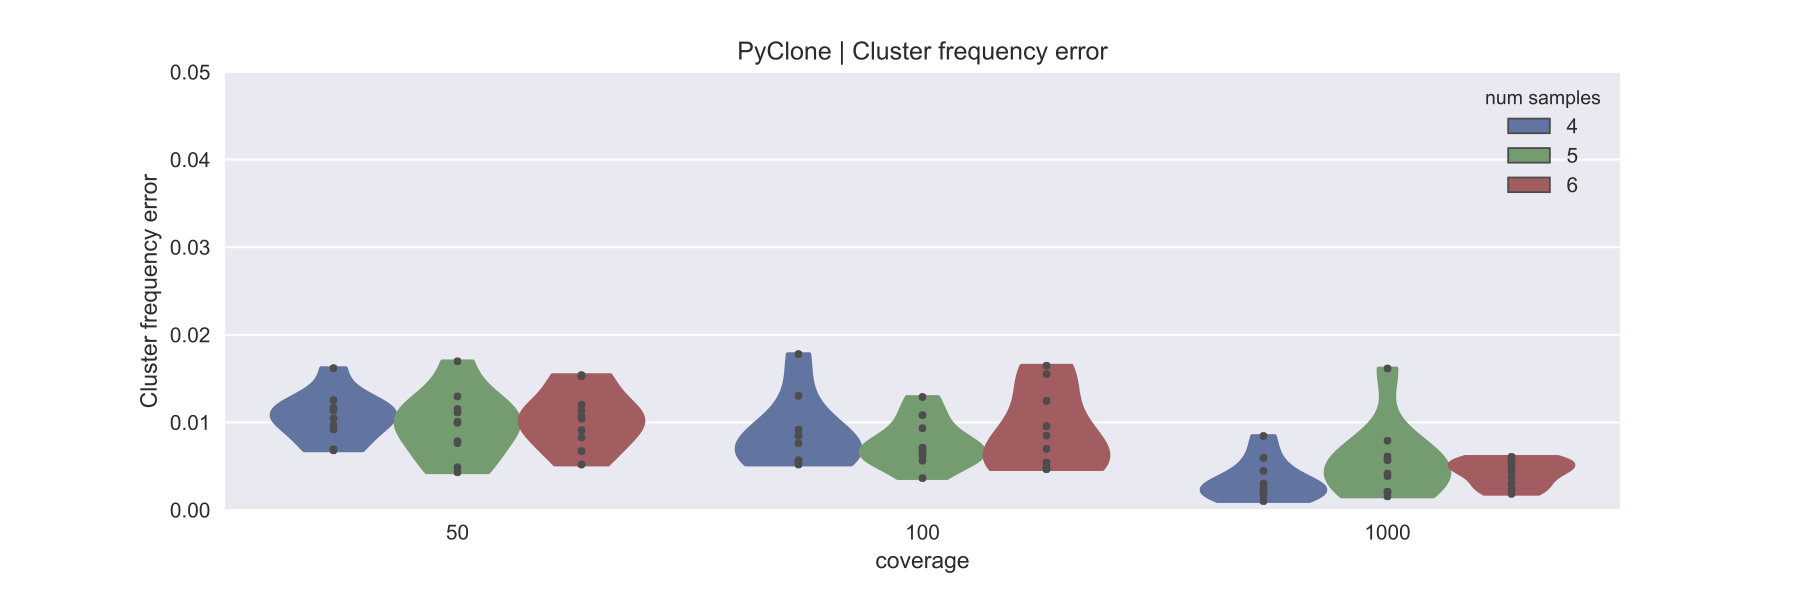
\includegraphics[scale=0.75]{PyClone_cluster_frequency_plot.png}}
\centerline{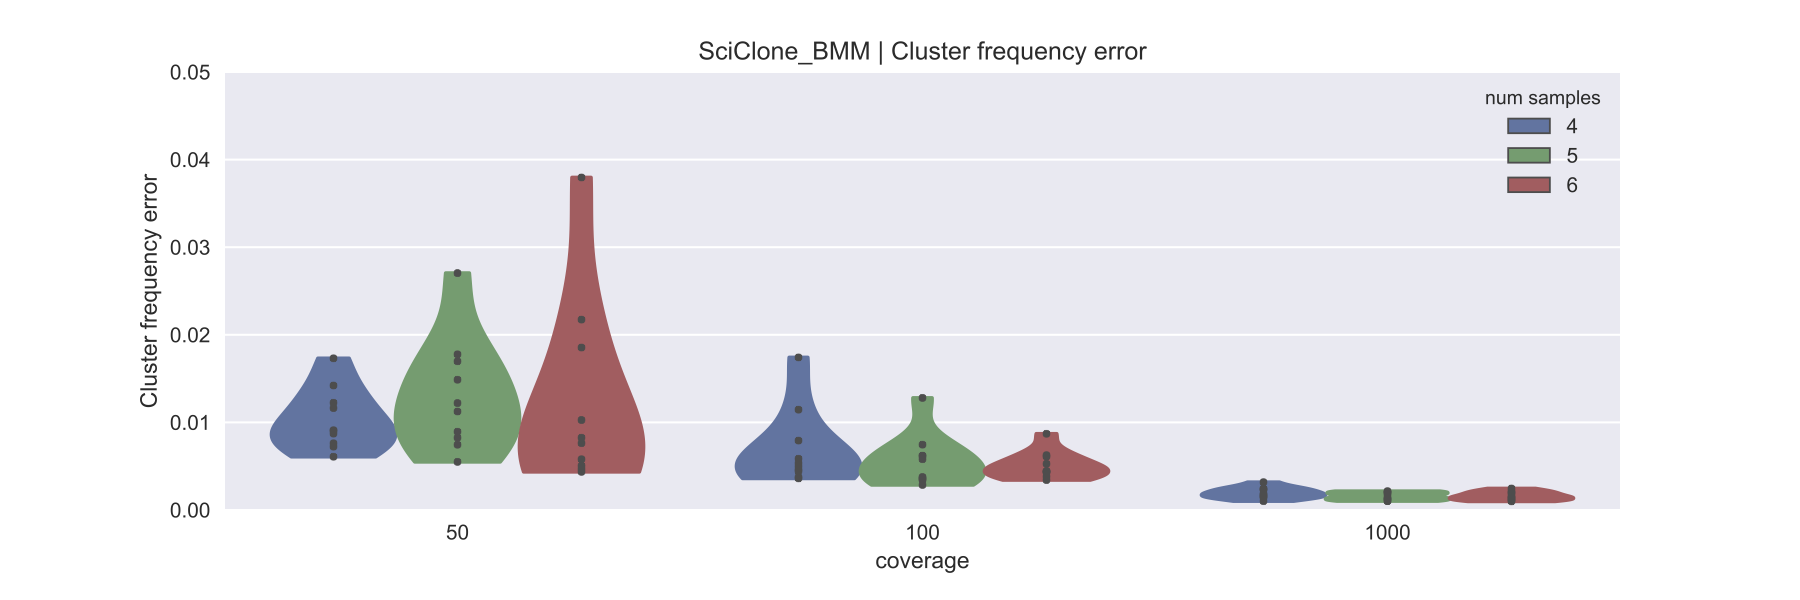
\includegraphics[scale=0.75]{SciClone_cluster_freq_error_plot.png}}
\caption{\emph{Comparison of cluster frequency errors on simulated data.}}
\label{fig:Heterogeneity}
\end{figure}

\newpage
\begin{figure}[h]
\centerline{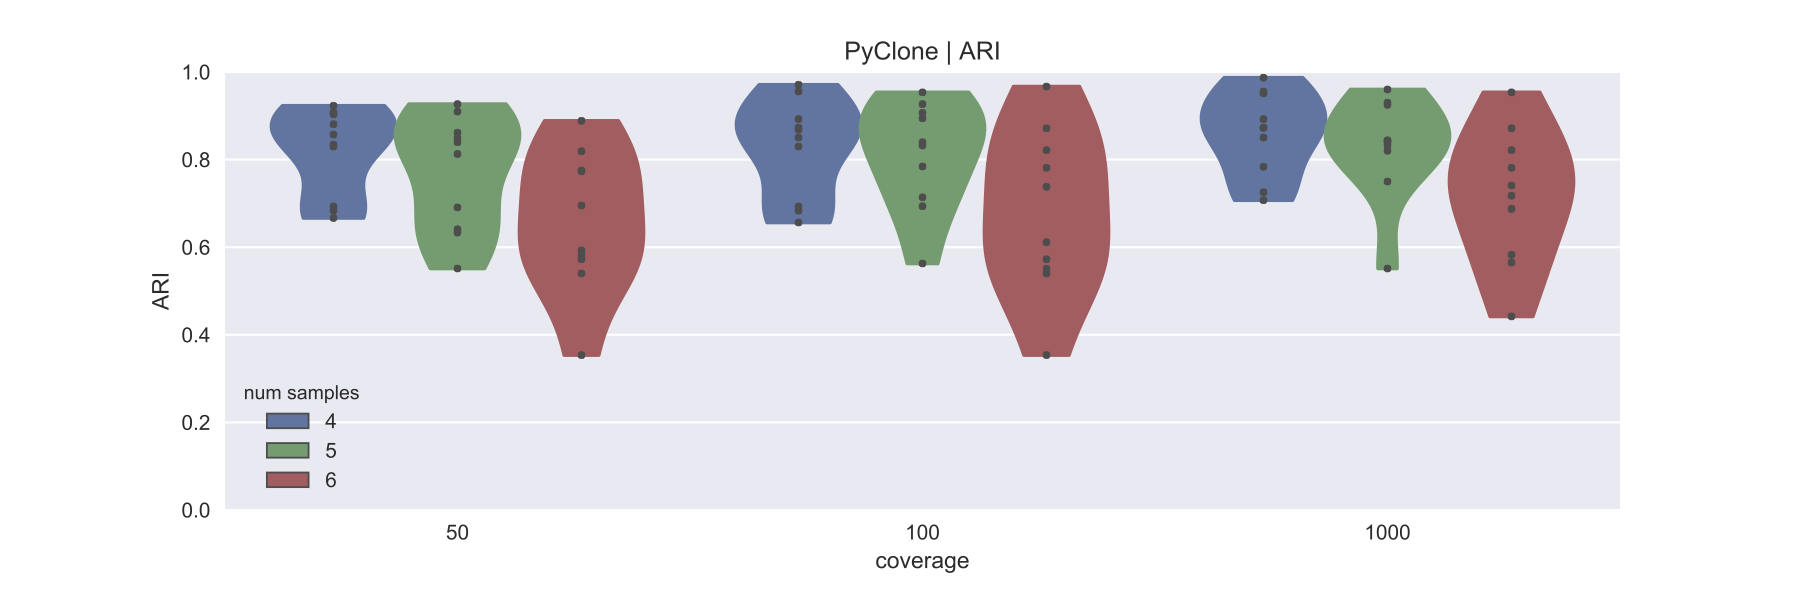
\includegraphics[scale=0.75]{PyClone_ARI.png}}
\centerline{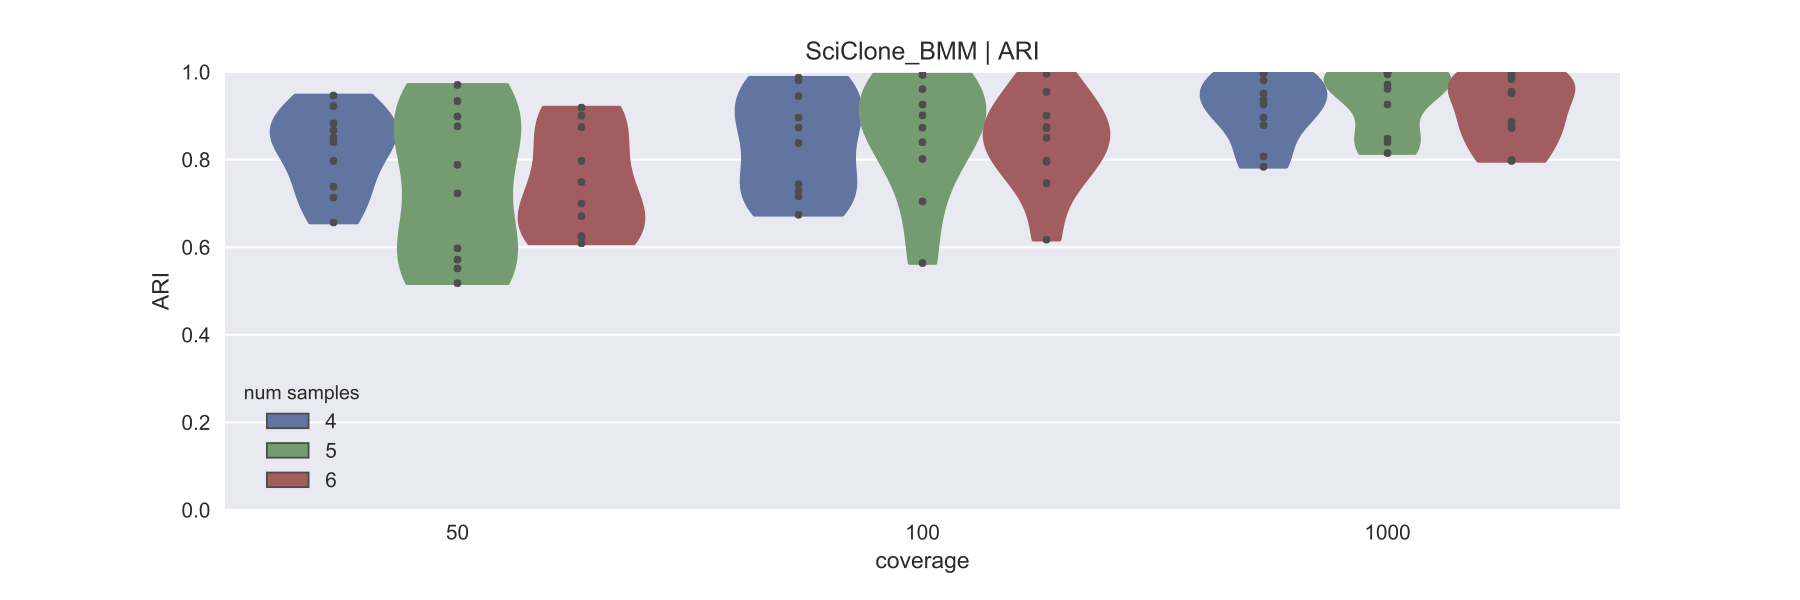
\includegraphics[scale=0.75]{SciClone_ARI.png}}
\caption{\emph{Comparison of adjusted Rand Index on simulated data.}}
\label{fig:Heterogeneity}
\end{figure}

\newpage
\begin{figure}[h]
\centerline{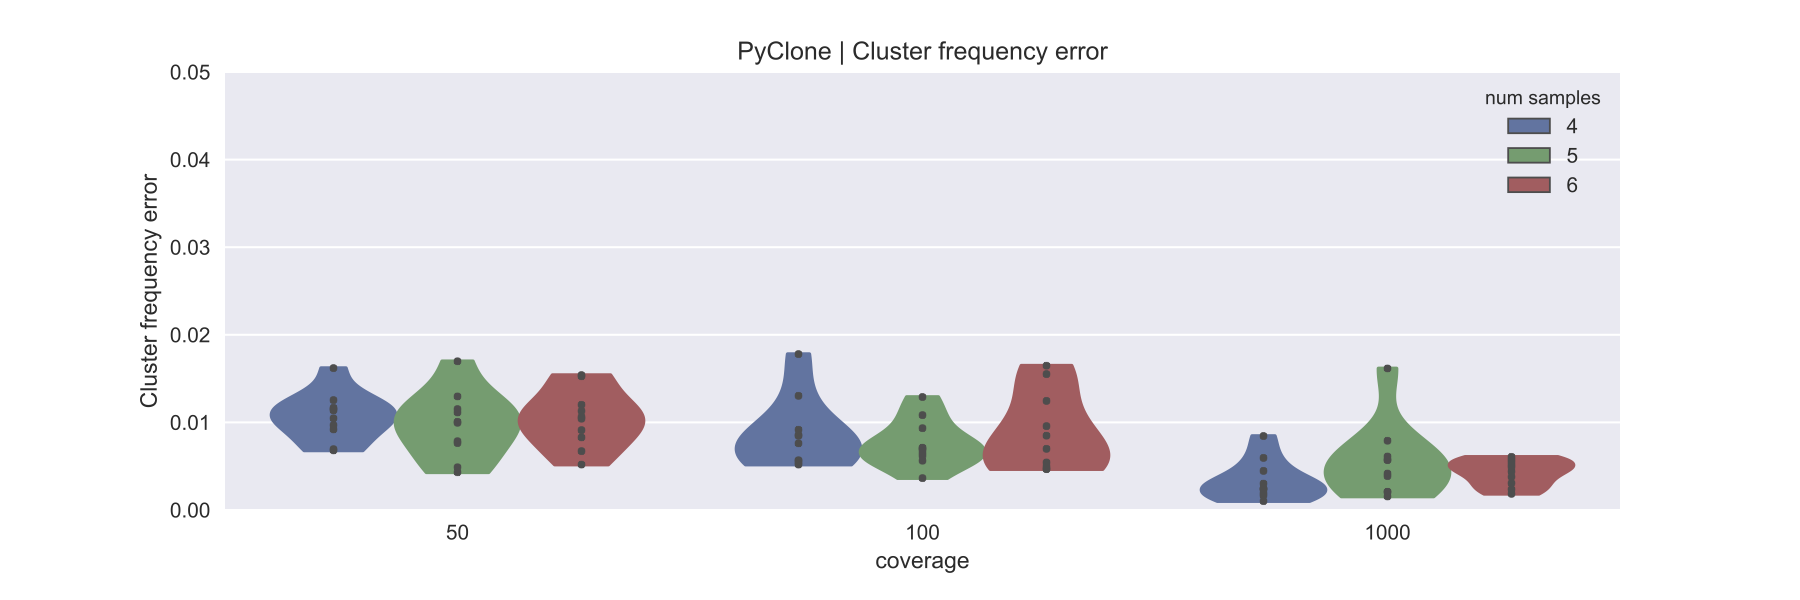
\includegraphics[scale=0.75]{PyClone_num_clusters.png}}
\centerline{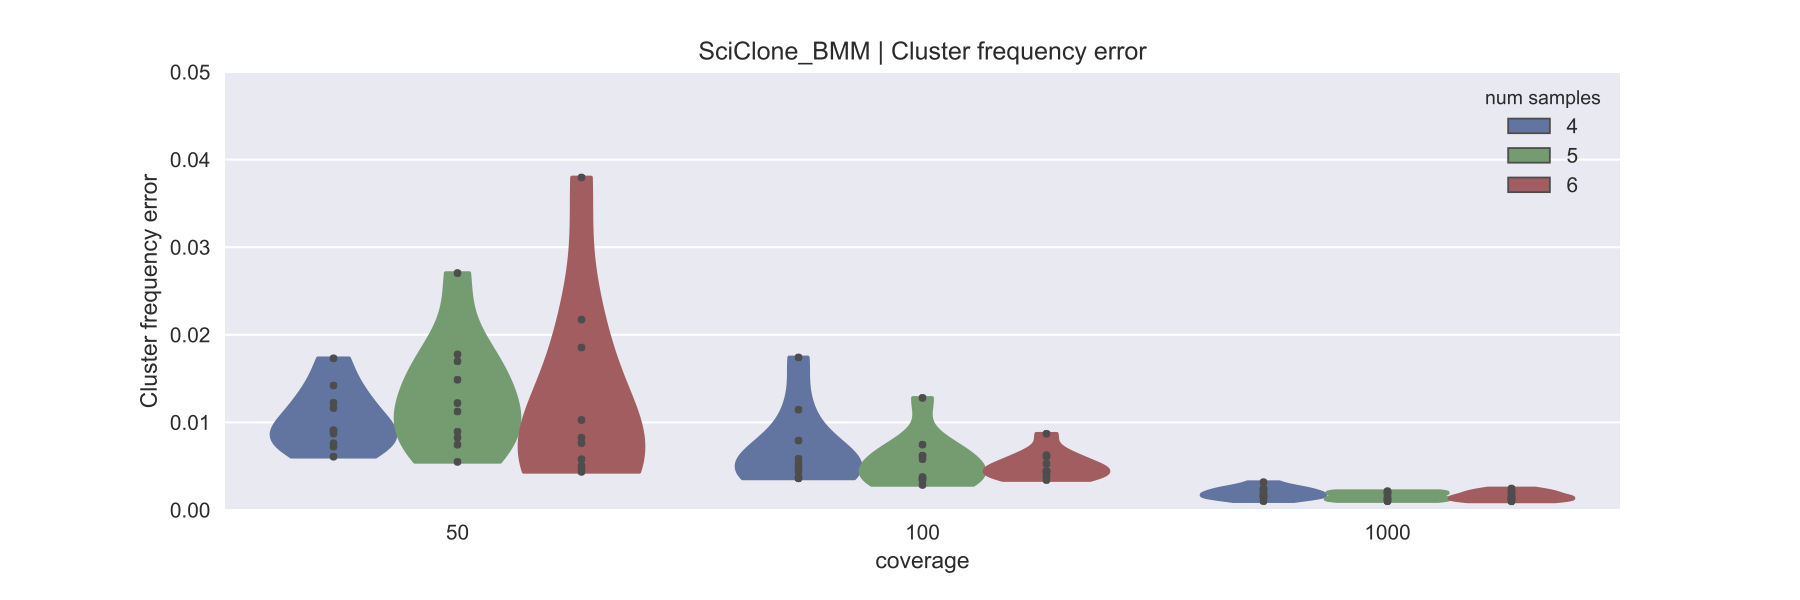
\includegraphics[scale=0.75]{SciClone_num_clusters.png}}
\caption{\emph{Comparison of cluster frequency errors on simulated data.}}
\label{fig:Heterogeneity}
\end{figure}



\begin{enumerate}
\item A beta plot for each type of clustering
\item Violin plots for each type of clustering 
\item One plot comparing the times
\end{enumerate}

+ Compare more samples vs more coverage

+ We expect VI to work faster: do a time plot. PyClone was run with 10000 iterations and a burn-in length of 1000 samples; these were the parameters recommended by PyClone's documentation. Figure X shows that the variational method is much faster than PyClone's MCMC inference, especially when more samples causes the dimensionality to increase. However, SciClone is faster because the model selection method makes variational inference with the finite-dimensional Dirichlet faster. Further, SciClone is implemented in R, which is faster than Python; the code for the DP/variational method could be optimized to be much faster.

\begin{itemize}
	\item Add to bnpy to get stochastic/memoized VI
	\item Use the results as input for other algorithms.
\end{itemize}

We have shown that the Dirichlet Process prior for the binomial mixture model with variational inference is a rigorous and efficient model and inference method for the SNV clustering problem. We were able to discover close to the correct number of clusters in most cases, with increasing sample size improving accuracy. As expected, variational inference worked much faster than MCMC methods. Writing the code in a faster language such as C or optimizing the code would  reduce the time gap between the nonparametric DP model and the parametric Dirichlet prior model.

The ultimate purpose of such clustering methods is to be used as part of a pipeline that reconstructs phylogenies

\appendix

\section{Allocation model update equations}
The coordinate ascent equations for the allocation model are standard \cite{Blei2006}, as they follow from the fact that the stick-breaking process is in the exponential family. The allocation model has variational parameters $\{\eta_{k0}, \eta_{k1}\}_{k=1}^K$ for the cluster proportions and $\{\hat{r}_{nk}\}_{n=1, k=1}^{N, K}$ for the cluster responsibilities. On each iteration, the coordinate update is
\begin{align}
\eta_{k1} &= 1 + \sum_n \hat{r}_{nk} = 1 + N_k \\
\eta_{k0} &= \gamma + \sum_n \sum_{j=k+1}^K \hat{r}_{nj} = N_k^>\\
\hat{r}_{nk} &\propto \exp(S_k) \\
\intertext{for $n = 1, \ldots, N$, $k=1, \ldots, K$, and where}
S_k &= \E_q[\log \bm{v}_k] + \sum_{i=1}^{k-1} \E_q \log(1 - \bm{v}_i) + \E_q[\log p(x_n | \alpha_{nk}, \beta_{nk})]
\intertext{and}
\E_q[\log \bm{v}_i] &= \Psi(\eta_{k0}) - \Psi(\eta_{k0} +\eta_{k1}) \\
\E_q[\log(1 -  \bm{v}_i)] &= \Psi(\eta_{k1}) - \Psi(\eta_{k0} +\eta_{k1})
\end{align}
The digamma functions come from the fact that derivative of the cumulant is the expectation, and the cumulant of a beta has gamma functions. Since the $\hat{r}_{nk}$ sum to 1 over $n=1, \ldots, N$ then we renormalize at every step as well.

\section{Observation model update equations}
Following the derivations in \cite{Hughes2015}, we derive the coordinate ascent equations for our observation model, taking advantage of the fact that $q(\bm{\phi}_k)$ is in the exponential family, which we show below.

\begin{claim}
$q(\bm{\phi}_k)$ is in the exponential family.
\begin{proof}
We know that
\begin{align*}
q(\bm{\phi}_k)  = \prod\limits_{m=1}^M q(\bm{\phi}_{mk}) = \prod\limits_{m=1}^M \mathrm{Beta}(\bm{\phi}_k | \alpha_{mk}, \beta_{mk}).
\end{align*}
The beta distribution is in the exponential family, with parameterization 
\begin{align}
\begin{split}
\mathrm{Beta}(\bm{\phi}_k |  \alpha_{mk}, \beta_{mk}) =  \frac{1}{\phi_{mk}(1 - \phi_{mk})} \exp \bigg(
		\begin{bmatrix}
			\log\phi_{mk} & \log(1 - \phi_{mk})
		\end{bmatrix}
		\begin{bmatrix}
			\alpha_{mk} \\ \beta_{mk}
		\end{bmatrix} \\
+ \log \Gamma(\alpha_{mk} + \beta_{mk}) - \log \Gamma(\alpha_{mk}) - \log\Gamma(\beta_{mk}) \bigg)
\end{split}
\end{align}
and thus $q(\bm{\phi}_k)$ is in the exponential family with the form
\begin{align*}
q(\bm{\phi}_k) = \left(\prod\limits_{m=1}^M \frac{1}{\phi_{mk}(1 - \phi_{mk})} \right) \exp\bigg(
			\begin{bmatrix}
				\begin{bmatrix}
				 \log\phi_{1k} & \log(1 - \phi_{1k} )
				\end{bmatrix} & \cdots &
				\begin{bmatrix}
				 \log\phi_{Mk} & \log(1 - \phi_{Mk})
				\end{bmatrix}
			\end{bmatrix}
			\begin{bmatrix}
				\begin{bmatrix}
				\alpha_{1k} \\ \beta_{1k} 
				\end{bmatrix} \\
				\vdots \\
				\begin{bmatrix}
				\alpha_{Mk} \\ \beta_{Mk}
				\end{bmatrix}
			\end{bmatrix} \\
			+ \sum\limits_{m=1}^M \log \Gamma(\alpha_{mk} + \beta_{mk}) - \log \Gamma(\alpha_{mk}) - \log\Gamma(\beta_{mk}) \bigg)
\end{align*}
where we have abused notation to show the tuple nature of the sufficient statistics. Thus, for our variational distribution $q(\bm{\phi}_k)$ we have
\begin{align}
\text{Natural parameters} &=  			\begin{bmatrix}
				\begin{bmatrix}
				\alpha_{1k} \\ \beta_{1k} 
				\end{bmatrix} \\
				\vdots \\
				\begin{bmatrix}
				\alpha_{Mk} \\ \beta_{Mk}
				\end{bmatrix}
			\end{bmatrix} \\
\text{Cumulant} &= \sum\limits_{m=1}^M \log \Gamma(\alpha_{mk} + \beta_{mk}) - \log \Gamma(\alpha_{mk}) - \log\Gamma(\beta_{mk}) \qedhere
\end{align}
\end{proof}
\end{claim}

\subsection{Exponential factorization of data model}
\vspace{-0.5cm}
\begin{align}
p(\bx_n | \bz_n) &= \prod\limits_{m=1}^M \mathrm{Bin}(v_{mn}; \phi_{mn}, d_{mn}) \nonumber \\
				 &= \prod\limits_{m=1}^M \exp\left(v_{mn} \log\left(\frac{\phi_{mn}}{1 - \phi_{mn}}\right) + (d_{mn} - v_{mn}) \log(1 - \phi_{mn}) \right) \nonumber \\				 		
\begin{split}
				&=\left( \prod\limits_{m=1}^M \binom{d_{mn}}{v_{mn}} \right)
				\exp\bigg( 
\begin{bmatrix}
         \log\left(\frac{\phi_{1n}}{1 - \phi_{1n}}\right) & \cdots & \log\left(\frac{\phi_{Mn}}{1 - \phi_{Mn}}\right)
        \end{bmatrix}\begin{bmatrix}
         v_{1n} \\ \vdots \\ v_{Mn}
        \end{bmatrix}  + \\
& \qquad \qquad\qquad\qquad\qquad\qquad \begin{bmatrix}
         \log\left(1 - \phi_{1n}\right) & \cdots & \log\left(1 - \phi_{Mn}\right)
        \end{bmatrix}      
                \begin{bmatrix}
         d_{1n} \\ \vdots \\ d_{Mn}
        \end{bmatrix} 
        \bigg)
        \end{split} \\
&=    \left( \prod\limits_{m=1}^M \binom{d_{mn}}{v_{mn}} \right)
			 \exp\bigg(
			\begin{bmatrix}
				\begin{bmatrix}
				 v_{1n} &  d_{1n}
				\end{bmatrix} & \cdots &
				\begin{bmatrix}
				 v_{Mn} &  d_{Mn}
				\end{bmatrix}
			\end{bmatrix}
			\begin{bmatrix}
				\begin{bmatrix}
					\log\left(1 - \phi_{1n}\right) \\ \log\left(\frac{\phi_{1n}}{1 - \phi_{1n}}\right)
				\end{bmatrix} \\
				\vdots \\
				\begin{bmatrix}
					\log\left(1 - \phi_{Mn}\right) \\ \log\left(\frac{\phi_{Mn}}{1 - \phi_{Mn}}\right)
				\end{bmatrix}
			\end{bmatrix} \bigg)\\
\end{align}
so that the sufficient statistics are
\begin{equation}
T(\bx_n) = 
\begin{bmatrix}
				\begin{bmatrix}
				 v_{1n} &  d_{1n}
				\end{bmatrix} & \cdots &
				\begin{bmatrix}
				 v_{Mn} &  d_{Mn}
				\end{bmatrix}
			\end{bmatrix}
\end{equation}

Thus, following (Hughes 2015) we have the following coordinate ascent updates for the observation model: (natural parameter plus sufficient statistic $S_k^{var}$ or $S_k^{ref}$)
\begin{align*}
\alpha_{mk} =  (\alpha_0 - 1) + \sum_{n=1}^N \hat{r}_{nk} \begin{bmatrix} v_{1n} \\ \vdots \\ v_{Mn} \end{bmatrix} \\
\beta_{mk} = (\beta_0 - 1) + \sum_{n=1}^N \hat{r}_{nk} \begin{bmatrix} d_{1n} \\ \vdots \\ d_{Mn} \end{bmatrix}
\end{align*}

\subsection{Sufficient statistics}
Define 
\begin{align}
S_k &= \sum_{n=1}^N \hat{r}_{nk} s(x_n) = \sum_{n=1}^N \hat{r}_{nk} \begin{bmatrix}
				\begin{bmatrix}
				 v_{1n} &  d_{1n}
				\end{bmatrix} & \cdots &
				\begin{bmatrix}
				 v_{Mn} &  d_{Mn}
				\end{bmatrix}
			\end{bmatrix} \\
N_k &= \sum_{n=1}^N \hat{r}_{nk} \\
N_k^> &= \sum_{k+1}^K N_k
\end{align}

\subsection{Obs Model Likelihoods}
\begin{align*}
\E_q[\log p(x_n | \alpha_{mk}, \beta_{mk})] &= \E_q[\log \left( \binom{d_{mn} + v_{mn}}{v_{mn}} (\bm{\phi}_k)^{v_{mn}} (1-\bm{\phi}_k)^{d_{mn}} \right)] \\
					&= \log\left(\binom{d_{mn} + v_{mn}}{v_{mn}}\right) + d_{mn} \E_q[\log \bm{\phi}_k] + v_{mn}\E_q[\log(1 -  \bm{\phi}_k)]
\intertext{where}
\E_q[\log \bm{\phi}_k] &= \Psi(\alpha_{mk}) - \Psi(\alpha_{mk} +\beta_{mk}) \\
\E_q[\log(1 -  \bm{\phi}_k)] &= \Psi(\beta_{mk}) - \Psi(\alpha_{mk} +\beta_{mk})
\end{align*}


\section{Computing the ELBO}

To test for convergence, we calculate the ELBO until the difference in ELBO between laps is less than some pre-specified number. For the purpose of this model, the convergence threshold was set to 1. Note that the ELBO is generally not a convex function, so we cannot make any guarantees about monotonicity.

Following \cite{Hughes2015}, the ELBO can be decomposed into three terms:
\begin{align*}
\ELBO \coloneqq \mathcal{L} = \mathcal{L}_{\text{Obs}} + \mathcal{L}_{\text{DP-Alloc}} + \mathcal{L}_{\text{Entropy}}
\end{align*}

\subsection{Observation model contribution to ELBO}
\begin{align}
\begin{split}
\mathcal{L}_{\text{Obs}} ={} & \E_{\bz, \bm{\phi}}[\log p(x | \bz, \bm{\phi})] + \E_\phi[\log p(\bm{\phi})] - \E_\phi[\log q(\bm{\phi})]
\end{split}\\
\begin{split}
							= {}& 	\sum\limits_{n=1}^N\sum\limits_{k=1}^K \hat{r}_{nk} \E_q[\log p(\bx_n | \bm{\phi}_k)] \\
							&+ \sum\limits_{k=1}^K\sum\limits_{m=1}^M \E_q[\log \bm{\phi}^0_k] \\
							&- \sum\limits_{k=1}^K\sum\limits_{m=1}^M \E_q[\log \bm{\phi}_k]
							\end{split}
\end{align}

\subsection{Allocation model contribution to ELBO}
\begin{align}
\begin{split}
\mathcal{L}_{\text{DP-Alloc}} ={} & \sum\limits_{k=1}^K c_{\text{Beta}}(1, \gamma) - c_{\text{Beta}}(\eta_{k1}, \eta_{k0})  \\
									&+ \sum\limits_{k=1}^K \left(N_k + 1 - \eta_{k1}) \E_q[\log \bm{u}_k]\right) \\
									&= \sum\limits_{k=1}^K \left(N_k^> + \gamma - \eta_{k0}\right) \E_q[\log(1 - \bm{u}_k)]
\end{split}
\intertext{where the expectations are defined above, and in (18), we showed that $c_\text{Beta}$ has the form}
c_\text{Beta}(\alpha, \beta) &= \log \Gamma(\alpha + \beta) - \log \Gamma(\alpha) - \log \Gamma(\beta)
\end{align}

\subsection{Entropy contribution to ELBO}
\begin{align*}
\mathcal{L}_{\text{Entropy}} = - \sum_{k=1}^K\sum_{n=1}^N \hat{r}_{nk} \log \hat{r}_{nk}
\end{align*}

\addcontentsline{toc}{section}{References}
\bibliographystyle{ieeetr}
\bibliography{bibliography}
\nocite{*}

\end{document}
